%% Template for a preprint Letter or Article for submission
%% to the journal Nature.
%% Written by Peter Czoschke, 26 February 2004
%%

\documentclass{nature}

\usepackage{graphicx}

%% make sure you have the nature.cls and naturemag.bst files where
%% LaTeX can find them

\bibliographystyle{naturemag}

\title{MedSavant: high-performance search engine for genetic variants}

%% Notice placement of commas and superscripts and use of &
%% in the author list

\author{Marc Fiume$^{1}$, Orion Buske$^{1}$, James Vlasblom$^{1}$, Eric Smith$^{1}$, Andrew Brook$^{1}$, Khushi Chachcha$^{2}$, Sergiu Dumitriu$^{1}$, Christian Marshall$^{3}$, Kym Boycott$^{4}$, Marta Girdea$^{1}$, Peter Ray$^{3}$, Gary Bader$^{5}$, Michael Brudno$^{1,3}$}

\begin{document}

\maketitle

\begin{affiliations}
 \item University of Toronto, Toronto, Ontario, M5S 1A1, Canada
 \item University of British Columbia, Vancouver, British Columbia, V6T 1Z4, Canada
 \item The Hospital for Sick Children, Toronto, Ontario, M5G 1X8, Canada
 \item University of Ottawa, Ottawa, Ontario, K1N 6N5, Canada
 \item The Donnelly Centre, Toronto, Ontario, M5S 3E1, Canada
\end{affiliations}

\begin{abstract}
Recent advancements in DNA sequencing technologies have economized the sequencing of individual genomes, creating potential to improve diagnostics and treatment for patients affected by genetic diseases. A significant challenge in utilizing these technologies in the clinical setting has been in the implementation of data analysis strategies that can be used to easily and efficiently identify causative genetic mutations from the large number of variants discovered through sequencing. A common approach is to annotate [1] and iteratively filter [2] potentially causal genetic mutations using ad-hoc combinations of computational scripts and their parameters; however, this method necessitates informatics expertise, is slow, non-interactive, and does not scale to the extent needed for clinical and other large-scale sequencing applications.
 
To facilitate the discovery of causative genetic mutations, we have developed MedSavant, an integrated solution for the storage, annotation, filtration, prioritization, and visual inspection of variants. It is entirely graphical, interactive, and scalable to manage datasets generated by large-scale sequencing projects. To accomplish this, the system employs big data analytics technologies optimized for genomic datasets that are capable of delivering the results of complex dynamic queries nearly instantaneously while using significantly less storage resources compared to the standard flat file equivalent [3].
 
The MedSavant platform was designed for use in large-scale research and clinical genome sequencing projects. We have created two MedSavant installations to demonstrate its use in these respective applications. The first installation contains over one billion unique variant entries from ZZZ of the 1000 Genomes Project [REF] individuals. This installation is publically accessible via an online portal. The second installation contains clinical data from 425 individuals from the FORGE Consortium, a set of projects whose aim is to discover the etiology of rare genetic disorders. Using MedSavant equipped with the internally-developed Mendel App, we independently discovered the causal gene in 16 tested FORGE Projects.
\end{abstract}

\section*{Motivation}
Next-generation DNA sequence analysis holds the promise of improving diagnostics and treatment for individuals affected with genetic diseases. A significant challenge to fulfilling its promise is in implementing data analysis strategies that can be used to easily and efficiently identify causative genetic mutations from the large number of variants discovered through sequencing in the clinical setting. A common approach is to annotate variants with informative metadata (e.g. genomic context, predicted harmfulness), filter for potentially causal genetic mutations based on complex criteria, and iteratively refine the previous steps after manual inspection of the results. This method utilizes a combination of ad-hoc and loosely integrated computational scripts that rely on flat files as the data-transfer medium.
 
This existing paradigm for genomic variant analysis, which involves serial processing of flat files with manual inspection as an endpoint, inherently requires a substantial amount of informatics expertise to run, is non-interactive and time-consuming, and thus does not scale to the extent needed for clinical and other large-scale sequencing applications. It is well appreciated in bioinformatics � and in other scientific domains � that visually-guided real-time exploration significantly aids the understanding of big datasets, as is evidenced by the success of tools like ABySS-Explorer[4], Savant Genome Browser[5], and Galaxy[6]. These tools deliver computationally-intensive analytics through accessible user interfaces. 

A few graphical applications for variant searching have previously been developed. VarB [7] enables visual exploration and rudimentary filtration of genomic variants based on size, quality, depth, and codon effect; but these features alone are not enough to resolve causal genetic mutations. VarSifter [8] and the SNP and Variation Suite [9], the latter being a commercial tool, are other desktop solutions for management, filtration, and visualization of genetic variants; however, their architecture places significant limitations on performance and restricts access to the data to a single computer. VarSifter loads the complete volume of genotyped variants into memory, and for this reason is practical only for exome analysis. As yet, there is an unmet need for accessible software to perform dynamic visual analyses of large volumes of genetic variant data detected through sequencing, with an emphasis on facilitating disease etiology discovery.
 
\section*{Introduction}
We introduce MedSavant, an integrated solution for the storage, annotation, filtration, prioritization, and visual inspection of variants that is entirely graphical, interactive, and scalable to manage datasets generated by large sequencing projects. MedSavant is a standalone client-server application that uses a custom high-performance database engine to store and perform faceted search queries on data. This design results in significantly improved performance and user-friendliness over standard flat file or client-side alternatives.
 
While standardized text-based flat file formats have commonly been used as a data-transfer medium for genomic datasets (e.g. BED, GFF, and the Variant Call Format (VCF) [10]) and enabled interoperability between computational tools, they do not facilitate faceted search - i.e. searches based on arbitrary metadata affiliated with the records.  This makes the interactive refinement of searches for causal genetic mutations difficult, as these are typically based on a complex set of quality, contextual, and other criteria that necessitate reprocessing these flat files whenever the search parameters change.  As a result, sets of candidate causal mutations often contain large numbers of poor quality or otherwise irrelevant variants that are frequently manually filtered, rather than resorting to further parameter refinement and reprocessing.  This problem is exacerbated as both the size and diversity of genomic datasets continue to increase.
 
\section*{MedSavant}
 
\subsection{Data and Annotation}
MedSavant employs the Infobright [REF] high-performance database and a custom query engine to quickly deliver results of faceted searches on genomic variant datasets. The database stores and compresses tables column-wise, and so uses substantially fewer resources and executes faster than flat file-based processing pipelines: MedSavant databases typically require 10-20X less disk space compared to raw VCF files, while simultaneously making it possible for common queries to execute in seconds or less. The facets that are searchable by MedSavant are numerous and customizable. They include both low-level genotype information (e.g. base quality, chromosome position) and high-level information (e.g. ethnicity, family, gender, phenotype). MedSavant also contains an internal annotation engine similar to ANNOVAR[11] and SnpEff[12] that automatically appends to all uploaded VCF files user-specified searchable annotations such as harmfulness prediction scores (e.g. SIFT[13], PolyPhen2[14]), allele frequencies from population sequencing studies (e.g. 1000 Genomes Project[15], NHLBI Exome Sequencing Project[16]), and ontology relationships (e.g. Gene Ontology[17], Human Phenotype Ontology[18], OMIM[19]). Table shows a list of data and annotations stored by MedSavant. Custom annotations are also supported.

\begin{table}
\centering
\caption{Data stored by MedSavant. Information stored for patients and variants can be extended. External datasets can be connected through Apps available on the MedSavant App Store.}
\medskip
\begin{tabular}{ccccc}
\hline
Patient & Genome & Annotations & Apps\\
\hline
Alternate Allele & Affected Status & Allele Frequencies (TGP, NHLBI) & WikiPathways\\
dbSNP IP & Family & Genes (RefSeq, UCSC) &  \\
Chromosome & Father & Ontology (GO, HPO, OMIM) &  \\
Position & Gender & Harmfulness (Polyphen-2, SIFT) &  \\
Genotype & Mother & more... &  \\
Quality & Patient ID &  &  \\
Reference Allele & Phenotype &  &  \\
Variant Type & more... &  &  \\
Zygosity &  &  &  \\
more... &  &  &  \\
\hline
\end{tabular}
\end{table}

\subsection{Search}
The MedSavant user interface manages remote authenticated access to the database, and offers a simple means for query construction and visualization of results. A list of search conditions and familiar widgets for tuning them are provided. Search conditions can be grouped, unioned, and intersected, yielding a very expressive query language. Queries can combine conditions based on both genotype and phenotype information; the synergistic use of both types of data allows for segmentation of mutations based on disease subgroups, an important functionality when investigating complex diseases like autism spectrum disorders or cancer. The user interface for faceted variant search is shown in Figure and specific examples of possible queries are provided in later sections. Searches can be constructed incrementally, one facet at a time, with nearly instant feedback about parameter effectiveness at each step. The dynamic provision of guidance during filter construction allows for rapid exploration of the parameter space and is one of the most significant time-saving advantages of the MedSavant platform. Moreover, MedSavant saves search states internally, producing no intermediary files that need to be managed by the user. Once a search has been fine-tuned, it can be saved and reused for reproducing results on different cohorts or on samples whose genotypes will be processed in the future.

\begin{figure}
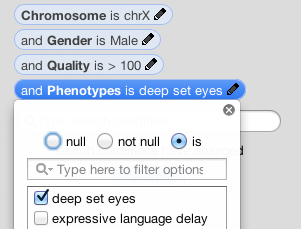
\includegraphics{search-genotype-phenotype} % this command will be ignored
\caption{Interface for specifying searches. Queries can be constructed based on both genotype and phenotype criteria.}
\end{figure}

\subsection{Inspection}
Candidate mutations can be manually inspected in various levels of detail as illustrated in Figure. The distribution of variants across the genome is depicted as a heatmap on a karyotypic ideogram. The distribution of variants can also be charted per searchable facet (as a histogram or pie chart), and between searchable facets (as a scatter plot). The full list of candidate variants is also represented in spreadsheet format with an associated Inspector that displays detailed information about selected variants, including all information contained in the original VCF file and a list of nearby genes. Further, the Inspector presents information regarding the function and relevance of nearby genes, including associated terms in the Gene Ontology, Human Phenotype Ontology, and OMIM. It also utilizes GeneMania[20], a service that finds related genes based on protein interaction and other networks, to suggest other genes to consider.


*Figure: Visualizing variant data at various resolutions. From top to bottom, a karyotypic heatmap shows the distribution of variants across chromosomes; a tabular view lists variants that pass the search criteria; the Inspector displays highly detailed information pertaining to the selected variant (left) and nearby genes (right); genome browser view of read alignments surrounding selected variant.

\subsection{Visualization}
It is often informative to inspect variants in their genomic context to ascertain their predicted functional consequence. Links in the Inspector offer the ability to navigate to and browse the genomic context of a candidate variant (including the corresponding read alignments from which the genotype prediction was initially made) using the embedded Savant Genome Browser. Savant is a next-generation genome browser that contains unique visualization modes for identifying and validating genetic variants. It contains multiple representations for exploring variant datasets: a traditional track view that displays variants per sample along a linear genomic coordinate system, and a streamlined non-linear display showing a condensed map, allele frequencies, and linkage disequilibrium derived from variable positions. Linking of the candidate variants list with the genome browser optimizes the inspection of results by removing the need to manually navigate to regions of interest as is required in traditional multi-tool workflows.

\subsection{Apps}
More data processing may be required to resolve disorders from filtered variants, for example by leveraging statistical analysis or by cross-sectioning the results with external datasets. MedSavant offers an Application Programming Interface (API) to foster integration with additional data processing tools developed by the community. Third-party Apps can leverage the MedSavant platform to access data, perform searches, do custom analyses, and present results within the graphical framework. A section of MedSavant, called the Clinic, is reserved for apps that perform push-button analyses for clinically-oriented workflows. Apps can be published to the MedSavant App Store, making useful additions to the platform available to all users. Two internally developed Apps are discussed below.

MedSavant Clinic
Figure: The MedSavant App Store provides access to third-party extensions to the platform. Apps can add complex search criteria, extend inspectors, or add novel visualizations or analyses. Clinically-oriented Apps are made available in the MedSavant Clinic.

\subsubsection{Enrichment App}
A single phenotype may be caused by genetic mutations at different positions in the genome, and so it is informative to aggregate potentially deleterious mutations based on genes, gene functions, and pathways, to concentrate analyses on relevant and noticeably perturbed biological functions. The Enrichment App aggregates variants by user-specified gene-lists, and terms in the Gene Ontology, Human Phenotype Ontology, or OMIM. Aggregation is a basic form of enrichment testing, and facilitates the process of identifying biological functions that are affected within the sequenced population, and ultimately understanding the genetic mechanisms of diseases.
 
\subsubsection{Mendel App}
Cohort, pedigree, and inheritance model information help to resolve the segregation of variants with genetic conditions. For example, VAAST[21] is a popular probabilistic disease-gene finder that can use such information to discover the causal gene(s) for genetic disorders given a modest number of genotyped samples. The Mendel App is an internally-developed disease-gene finder that adds the ability to resolve disorders through case-control and pedigree analysis. Given complete pedigree information, Mendel can also perform segregation based on known inheritance models. Once installed Mendel is made available in the MedSavant Clinic; a clinical application of this utility is discussed in the section that follows.
 
\section*{Case Study}
 
The MedSavant platform was designed for use in both large-scale research and clinical genome sequencing projects. We have created two MedSavant installations to demonstrate its use in these respective applications. The first installation contains over one billion unique variant entries from ZZZ of the 1000 Genomes Project individuals. This installation is publically accessible via an online portal. The second installation contains clinical data from 425 individuals from the FORGE Consortium, a set of projects whose aim is to discover the etiology of rare genetic disorders. Using MedSavant equipped with the internally-developed Mendel App, we independently discover the causal gene in 16 tested FORGE Projects.

FORGE is a national consortium whose mission is to discover the etiology of a large number of rare genomic conditions. For example, Joubert syndrome is a rare brain malformation characterized by the absence or underdevelopment of the cerebellar vermis, an area of the brain that controls balance and coordination [REF]. Common symptoms in infants affected by Joubert syndrome include mental retardation, inability to coordinate voluntary muscle movements (ataxia), jerky eye movements (oculomotor apraxia), rapid breathing (hyperpnea), and decreased muscle tone (hypotonia). Joubert syndrome occurs in about 1 in 100,000,000 births, although there is a relatively high prevalence in the French-Canadian population, with several founder effects noted. SNP genotyping was previously performed on 9 affected individuals from seven families living in the Lower St. Lawrence region, and from this data it was previously discovered that mutations in C5orf42 cause Joubert syndrome in this French Canadian population [REF].

20 FORGE disorders, including Joubert syndrome, were chosen for validation with Mendel based on the availability of genotype data, pedigree data, and consistency in their sequencing and genotyping pipelines. For each of the chosen disorders, genomic DNA from patients was captured using the Agilent SureSelect 50 Mb oligonucleotide library and sequenced with Illumina HiSeq2000, yielding 100bp paired-end reads. Putative PCR-generated duplicates were removed from the raw read data using Picard [REF], alignment was performed using the Burrows-Wheeler Aligner (BWA) [Ref], and custom scripts for SamTools [REF], Pileup [REF], and varFilter [REF] were used to call variants. 

We created a MedSavant database containing genotypes from all FORGE projects for which data was available, comprising 425 individuals and 138,640,418 variants identified from their samples. MedSavant was used to specify stringent quality filters (minimum coverage of 3; support from both strands; quality � 50 for indels and � 30 for SNVs; either exonic, splicing, or in UTR; allele frequency � 0.05) yielding 427,765 variants. For each of the 20 chosen FORGE projects, Mendel was used to identify variants that segregate with the disorder using the remaining individuals, including family members of affected individuals and unaffected individuals from other projects, as controls. For Joubert syndrome, the Mendel expression shown in Figure produced missense and splicing mutations in C5orf42, with no other results. The positions of mutations identified by Mendel were manually inspected using the built-in genome browser. All 9 of the affected individuals were found to carry compound heterozygous mutations in this gene unlike any of the controls.

Figure: Mendel expression used to identify harmful variants in C5orf42 (top), an independent discovery of the gene�s involvement in causing Joubert syndrome in 9 French-Canadians. The expression yielded variants in this gene only (bottom).

Using a similar workflow the causal gene was independently discovered for 16 of the 20 chosen disorders, listed in Table. Of the 4 disorders which were not rediscovered, the causal variant either did not pass the aforementioned quality filters or the causal variant was not included in the provided VCF files (e.g. a causal CNV was identified by other means). A summary of the Mendel expressions used for each confirmed disorder is provided in the Supplementary Information.

\section*{Conclusion and Future Work}
The potential to gain new insights into genetic disease is currently encumbered by significant challenges in the data analysis methodologies that can be used to easily, efficiently, and intelligently identify causative genetic mutations from the large number of variants discovered through sequencing. Existing approaches either rely on complicated computational pipelines that include manual inspection only as an endpoint, or are desktop-based solutions that do not scale well for medium-to-large sequencing experiments. MedSavant is a genomic variant search engine built upon the client-server paradigm designed to meet the demands of even large population sequencing studies. It unifies the storage, annotation, filtration, prioritization, and visual inspection of variants into a powerful yet simple-to-use graphical interface that is designed for users with all levels of computational expertise, with demonstrated utility in both clinical and research settings.
 
We are actively developing a version of the software that is capable of distributing queries across private computational clusters or across multiple instances running in the cloud, furthering increasing the performance and scalability of the platform. We also intend to work with third-party developers to create additional MedSavant Apps that leverage the platform�s resources to deliver cutting-edge statistical and visual analytics of genomics data.

%% Put the bibliography here, most people will use BiBTeX in
%% which case the environment below should be replaced with
%% the \bibliography{} command.

% \begin{thebibliography}{1}
% \bibitem{dummy} Articles are restricted to 50 references, Letters
% to 30.
% \bibitem{dummyb} No compound references -- only one source per
% reference.
% \end{thebibliography}

\bibliographystyle{naturemag}
\bibliography{sample}


%% Here is the endmatter stuff: Supplementary Info, etc.
%% Use \item's to separate, default label is "Acknowledgements"

\begin{addendum}
 \item Put acknowledgements here.
 \item[Competing Interests] The authors declare that they have no
competing financial interests.
 \item[Correspondence] Correspondence and requests for materials
should be addressed to A.B.C.~(email: myaddress@nowhere.edu).
\end{addendum}

%%
%% TABLES
%%
%% If there are any tables, put them here.
%%

\begin{table}
\centering
\caption{This is a table with scientific results.}
\medskip
\begin{tabular}{ccccc}
\hline
1 & 2 & 3 & 4 & 5\\
\hline
aaa & bbb & ccc & ddd & eee\\
aaaa & bbbb & cccc & dddd & eeee\\
aaaaa & bbbbb & ccccc & ddddd & eeeee\\
aaaaaa & bbbbbb & cccccc & dddddd & eeeeee\\
1.000 & 2.000 & 3.000 & 4.000 & 5.000\\
\hline
\end{tabular}
\end{table}

\end{document}
